%%%%%%%%%%%%%%%%%%%%%%%%%
\section{Introduction}
\label{sec-intro}
%%%%%%%%%%%%%%%%%%%%%%%%%

Let us recall the history of the Hecke algebra from the perspectives of algebraization and categorification.

%%%%%%%%%%%%
\subsection{The Hecke algebra by generators and relations}
%%%%%%%%%%%%

Let $G$ be a split finite reductive group over a finite field $\mathbb{F}_q$, and let $B \subset G$ be a Borel subgroup.  A fundamental object in representation theory is the Hecke algebra
\[
\mathrm{Fun}_{B \times B}(G, \mathbb{C})
\]
of $B$-biinvariant complex valued functions on $G$, with multiplication given by convolution. This algebra first emerged when studying the irreducible complex characters of $G$, but has gone on to play an essential role in many (at times unexpected) branches of representation theory.

Iwahori \cite{Iwahori} made the crucial observation that the Hecke algebra admits a description which is ``independent" of the size $q$ of the base field and only depends on the Weyl group.
Fix a maximal split torus $T \subset B$ and let $(W,S)$ denote the Weyl group and its simple reflections. Using the Bruhat decomposition
\[
G = \bigsqcup_{w \in W} BwB
\]
it follows that the Hecke algebra has a basis given by indicator functions of the subsets $BwB \subset G$. Now let $\HB$ be the free $\Zvv$-module with basis $\{ T_w \; | \; w \in W \}$. There is a unique algebra structure on $\HB$ determined by
\[
T_wT_s = \begin{cases} T_{ws} & \text{if $ws > w$,} \\ (v^{-2}-1)T_w + v^{-2}T_{ws} & \text{if $ws < w$}. \end{cases}
\]
Writing $\HB_{\FM_q} \define \HB \otimes \CM$ for the specialization of $\HM$ at $v^{-1} \mapsto \sqrt{|\FM_q|} \in \CM$, we have an isomorphism of algebras
\[
\HB_{\FM_q} \stackrel{\sim}{\longto} \mathrm{Fun}_{B \times B}(G, \mathbb{C})
\]
sending $T_w$ to the indicator function of $BwB \subset G$. (One could define $\HB$ over $\ZM[q^{\pm 1}]$. The introduction of a square root of $q$ is a notational convenience which becomes important later.)
Furthermore, the algebra $\HB$ is generated by the elements $\{T_s \; | \; s \in S \}$, modulo the quadratic relation \[ (T_s + 1)(T_s - v^{-2}) = 0\] and the braid relations
\[ \ubr{T_sT_t \dots }{m_{st}} = \ubr{T_tT_s \dots}{m_{st} }
\] where $m_{st}$ denotes the order of $st$ in $W$.

This presentation of the Hecke algebra has paved the way for an algebraic study of its representation theory. An immediate consequence is that the Hecke algebra may be defined for any
Coxeter system, whether or not it arises as the Weyl group of a reductive algebraic group (or suitable generalizations such as an affine or Kac-Moody groups). Thus was the Hecke algebra
freed from its concrete realization as a convolution algebra.

%%%%%%%%%%%%%%
\subsection{The Hecke category}
%%%%%%%%%%%%%%

Beginning with the seminal work \cite{KaL1} of Kazhdan and Lusztig it was realised that the Hecke algebra admits a categorification, which has come to be known as the Hecke category. 
 According to Grothendieck's function-sheaf dictionary, the algebra of $B$-biinvariant functions on $G$ should be categorified by some version of $B$-biequivariant sheaves on $G$. For concreteness, we now suppose that $G$ is a complex reductive group with Borel subgroup $B$ and maximal torus $T \subset G$. The Hecke category (in its simplest geometric incarnation) is the additive subcategory of semi-simple complexes
\[
\HC \subset D^b_{B \times B}(G, \CM)
\]
in the equivariant derived category of $B$-biequivariant sheaves on $G$. In other words, the objects of $\HC$ are direct sums of shifts of various $\ic_w \define \ic(\overline{BwB})$, the equivariant intersection cohomology complexes of $B \times B$-orbits. There is a monoidal structure $*$ on $D^b_{B \times B}(G,\CM)$ given by convolution, and it preserves $\HC$, thanks to the Decomposition Theorem and the compactness of $G/B$. Therefore the split Grothendieck group $[\HC]$ of $\HC$ has a $\Zvv$-algebra structure (the $\ZM[v^{\pm 1}]$ structure is given by $v[\FC] = [\FC[1]]$). The key result is an isomorphism of $\Zvv$-algebras
\[
\HB \stackrel{\sim}{\longto} [\HC]
\]
which sends the Kazhdan-Lusztig basis element $\underline{H}_w \in \HB$ to $[\ic_w]$. The Kazhdan-Lusztig basis also has a purely algebraic definition, and it was quickly realised that this definition mimics the defining properties of an intersection cohomology complex.

%%%%%%%%%%%%%%
\subsection{Soergel bimodules}
%%%%%%%%%%%%%%

Just as Iwahori gave an intrinsic construction of the Hecke algebra so too would Soergel give one of the Hecke category.

Let $\hg$ denote the Lie algebra of $T$ and $R$ the regular functions on $\hg$, graded so that $\hg^*$ is in degree two. We have a canonical identification of equivariant cohomology groups
(the ``Borel isomorphism'') \[ R = H^{\bullet}_T(\pt) = H^{\bullet}_B(\pt). \] In particular, the hypercohomology of any object in $ D^b_{B \times B}(G, \CM)$ is naturally a graded module
over $H^{\bullet}_{B \times B}(\pt) = R \otimes_{\CM} R$. Because $R$ is commutative, we may regard any $R \otimes R$-module as an $R$-bimodule. Hence hypercohomology can be see as a functor to 
$R-\Bim$, the category of graded $R$-bimodules.

Soergel's first key observation is that hypercohomology \[ \HM^{\bullet}_{B \times B} : \HC \to R-\Bim \] is fully-faithful and monoidal (that is $\HM^{\bullet}_{B \times B}(\FS * \GS) \cong \HM^{\bullet}_{B \times B}(\FS) \otimes_R \HM^{\bullet}_{B \times B}(\GS)$ for $\FS, \GS \in \HC$). It follows that the Hecke category is
equivalent to its essential image. His second key observation is that the Decomposition Theorem gives an alternative description of the intersection cohomology complexes. That is,
$\ic_w$ is the unique summand of $\ic_s * \ic_t * \cdots * \ic_u$ (for a reduced expression $st\ldots u$ of $w$) which does not appear in the analogous convolution for any shorter reduced
expression. This description arises from the Bott-Samelson resolution of a Schubert variety, and so we call it the ``Bott-Samelson description" of an intersection cohomology complex.

Note that $W$ acts on $\hg$ and hence on $R$ via graded algebra automorphisms. It is easy to calculate that
\[
\HM^{\bullet}_{B \times B} (\ic_s) = B_s \define R \otimes_{R^s} R(1)
\]
where $R^s \subset R$ denotes the subalgebra of $s$ invariants in $R$, and $(1)$ denotes the grading shift. From this, Soergel obtained the following elementary description of $\HC$: it is equivalent to the smallest full additive monoidal Karoubian graded subcategory of $R-\Bim$ containing $B_s$ for all $s \in S$. This category is by definition the category $\SBim$ of \emph{Soergel bimodules}. By the above discussion, hypercohomology yields an equivalence of graded monoidal categories:
\[
\HC \stackrel{\sim}{\longrightarrow} \SBim.
\]

% Concretely, the indecomposable Soergel bimodules are the direct summands (as graded $R$-bimodules) of the graded $R$-bimodules of the form
% \[
% B_{s} \otimes_R B_t \otimes_R \dots \otimes_R B_u[m] = R \otimes_{R^s} R \otimes_{R^t} \dots \otimes_{R^u} R[m + n]
% \]
% where $st \dots u$ is any sequence of simple reflections of length $n$ and $m \in \ZM$.

In this setting, $\SBim$ is just another incarnation of the Hecke category. However, as Soergel pointed out, this algebraic description allows one to define the Hecke category for arbitrary Coxeter systems, for which there is no suitable geometric context. In \cite{Soe3} Soergel imitates the above definition of $\SBim$ starting with an appropriate (``reflection faithful'') representation $\hg$ of $W$, which plays the role of the representation of $W$ on the Lie algebra $\hg$ of $T$. With $\SBim$ defined as above, Soergel then constructs an isomorphism of $\Zvv$-algebras
\[
\HB \stackrel{\sim}{\longto} [\SBim].
\]
In analogy to the Bott-Samelson description of intersection cohomology complexes in $\HC$, Soergel proves that the indecomposable bimodules $\{B_w\}$ in $\SBim$ are in bijection with $W$, and that $B_w$ is the unique summand of $B_s \ot B_t \ot \cdots \ot B_u$ (for a reduced expression of $w$) which does not appear for a shorter expression. These results are known as Soergel's Categorification Theorem.

For a Weyl group, one can prove Soergel's Categorification Theorem easily by transferring known facts about $\HC$ to $\SBim$ using hypercohomology. Soergel's proof for the general case is much trickier, but relies only on commutative algebra. Soergel proves his results for reflection faithful representations of a Coxeter system over an infinite field of characteristic $\ne 2$.

Soergel's theory (or the Bott-Samelson description of $\HC$) states that the objects of $\SBim$ are generated by the objects $B_s$. Moreover, there are isomorphisms between objects in $\SBim$ which lift the quadratic and braid relations of the Hecke algebra. (One should not categorify the Iwahori presentation given above, but a presentation using the Kazhdan-Lusztig generators which we will describe below.)  Heuristically speaking, this is the categorical analogue of Iwahori's algebraization of $\HB$, on the level of objects. However, in $\HC$ or $\SBim$ there is a whole new layer of structure, with no analogue in the Hecke algebra: the composition of morphisms.

%%%%%%%%%%%%%%%
\subsection{Soergel bimodules by generators and relations}
%%%%%%%%%%%%%%%

A \emph{Bott-Samelson bimodule} is a bimodule of the form $B_{\un{w}} \define B_s \ot_R B_t \ot_R \cdots \ot_R B_u$ for an expression $\un{w}=st\dots u$. They form a full
monoidal subcategory of $R-\Bim$, which we denote $\BSBim$. By definition, any Soergel bimodule is a direct sum of shifts of summands of bimodules in $\BSBim$. Said another way, the
category of Soergel bimodules $\SBim$ is the Karoubi envelope of (the additive, graded envelope of) $\BSBim$. The upshot is that in order to describe the category of Soergel bimodules it
is enough to describe the monoidal category of Bott-Samelson bimodules. This is an easier problem because (in contrast to Soergel bimodules) one has concrete combinatorial realizations of
the objects in $\BSBim$.

In this paper we describe the monoidal category of Bott-Samelson bimodules by
generators and relations. (There is one caveat, involving standard parabolic subgroups of type $H_3$ which shall be discussed in section \ref{threecolorintro} below.) Such a description has already been given by Libedinsky
\cite{LibRA} in the right-angled case (i.e. when $m_{st} \in \{2,\infty\}$), in type $A$ by the first author and Khovanov \cite{EKh}, and in dihedral type by the first author in
\cite{EDihedral}. This is the next step in the algebraization of $\HC$, freeing the category of Soergel bimodules from its realization as a full subcategory of a bimodule category. Said
another way, in this paper we give a $2$-presentation of $\BSBim$, in analogy to the $1$-presentation of $\HB$ given by Iwahori. Our presentation will use the technology of planar
diagrammatics.

We assign a color to each element of $S$, which allows us to encode a Bott-Samelson bimodule as a sequence $\un{w}$ of colored dots ordered on
a line. A morphism between Bott-Samelson bimodules will be given by a linear combination of isotopy classes of decorated graphs embedded in the planar strip $\RM \times [0,1]$. The edges
in these graphs will be colored, and may run into the bottom boundary $\R \times \{0\}$ or the top boundary $\R \times \{1\}$, yielding a sequence of colored dots on each boundary. A
morphism from $B_{\un{w}}$ to $B_{\un{y}}$ will have bottom boundary $\un{w}$ and top boundary $\un{y}$. For example, the following planar diagram
\igc{1}{morphismexample}
represents a map from $rgrgrgbr$ to $grbgrbr$.

For the moment, let us ignore the notion of isotopy classes of graphs, and consider instead diagrams which can be constructed from horizontal and vertical concatenation of the following generators. Here is a list of generating morphisms, their degrees and the maps of Soergel bimodules which they represent:
\[
\begin{array}{cccc}
\begin{array}{c}\tikz[scale=0.5]{\draw[dashed] (3,0) circle (1cm);
\draw[color=blue] (3,-1) to (3,0);
\node[circle,fill,draw,inner sep=0mm,minimum size=1mm,color=blue] at (3,0) {};}\end{array}& \text{deg 1} & B_{\color{blue}s} \to R  & f \otimes g \mapsto fg 
\\
\begin{array}{c}\tikz[scale=0.5]{\draw[dashed] (3,0) circle (1cm);
\draw[color=blue] (3,1) to (3,0);
\node[circle,fill,draw,inner sep=0mm,minimum size=1mm,color=blue] at (3,0) {};}\end{array}
& \text{deg 1}&
R \to B_{\color{blue}s}  & 1 \mapsto \frac{1}{2}(\alpha_s \otimes 1 + 1
  \otimes \alpha_s)
\\
\begin{array}{c}\tikz[scale=0.5]{\draw[dashed] (0,0) circle (1cm);
\draw[color=blue] (-30:1cm) -- (0,0) -- (90:1cm);
\draw[color=blue] (-150:1cm) -- (0,0);}\end{array}
&  \text{deg -1} & 
B_{\color{blue}s} B_{\color{blue}s} \to B_{\color{blue}s}  & 1 \otimes g \otimes 1 \mapsto \partial_s g
  \otimes 1
\\

\begin{array}{c}\tikz[scale=0.5]{\draw[dashed] (0,0) circle (1cm);
\draw[color=blue] (30:1cm) -- (0,0) -- (-90:1cm);
\draw[color=blue] (150:1cm) -- (0,0);}\end{array}
&  \text{deg -1} & B_{\color{blue}s} \to B_{\color{blue}s} B_{\color{blue}s}  & 1 \otimes 1 \mapsto 1 \otimes 1
  \otimes 1 \\
\begin{array}{c}\tikz[scale=0.5]{\draw[dashed] (0,0) circle (1cm);
\node at (0,0) {$f$};}\end{array}
&  \text{deg f} &
R \to R  & 1 \mapsto f
\\
\begin{array}{c}\tikz[scale=0.5]{\draw[dashed] (0,0) circle (1cm);
\draw[color=blue] (0,0) -- (22.5:1cm);
\draw[color=blue] (0,0) -- (67.5:1cm);
\draw[color=blue] (0,0) -- (112.5:1cm);
\draw[color=blue] (0,0) -- (157.5:1cm);
\draw[color=blue] (0,0) -- (-22.5:1cm);
\draw[color=blue] (0,0) -- (-67.5:1cm);
\draw[color=blue] (0,0) -- (-112.5:1cm);
\draw[color=blue] (0,0) -- (-157.5:1cm);
\draw[color=red] (0,0) -- (0:1cm);
\draw[color=red] (0,0) -- (45:1cm);
\draw[color=red] (0,0) -- (90:1cm);
\draw[color=red] (0,0) -- (135:1cm);
\draw[color=red] (0,0) -- (180:1cm);
\draw[color=red] (0,0) -- (-45:1cm);
\draw[color=red] (0,0) -- (-90:1cm);
\draw[color=red] (0,0) -- (-135:1cm);
}\end{array}
&  \text{deg 0}&  \ubr{B_{\color{blue}s}B_{\color{red}t} \dots }{m_{st}}  \to \ubr{B_{\color{red}t} B_{\color{blue}s} \dots }{m_{st}}    & 
\end{array}
\]
In the above, $\alpha_s$ denotes a fixed choice of equation for the hyperplane fixed by $s$, and $\pa_s$ denotes the Demazure operator $\pa_s(f) \define (f - sf)/\a_s$. We refer to the first two morphisms as \emph{dots}, the second two morphisms as \emph{trivalent vertices}, and the final morphism as the \emph{$2m_{st}$-valent vertex}.

We have not given a formula for the $2m_{st}$-valent vertex, as it is both difficult and unenlightening to write down explicitly in general. It can be described conceptually as follows. Let $B_{s,t}$ denote the indecomposable Soergel bimodule indexed by the longest element of the (finite) rank two parabolic subgroup generated by $s$ and $t$.  The bimodules $B_{\color{blue}s}B_{\color{red}t} \dots $ and $B_{\color{red}t} B_{\color{blue}s} \dots $ each contain $B_{s,t}$ as a summand with multiplicity one. The $2m_{st}$-valent vertex is the projection and inclusion of this common summand. (This determines the morphism up to a scalar, and there is a simple way to fix this choice of scalar.)

It is a result due to Libedinsky \cite{Lib} that these morphisms generate all morphisms between Bott-Samelson bimodules. In this paper we determine the relations which they satisfy. Let us
call a subset $J \subset S$ \emph{finitary} if the corresponding parabolic subgroup is finite. In the Iwahori presentation of $\HB$ for a Coxeter system, there is a generator
$T_s$ for each $s \in S$, i.e. for each finitary subset of rank $1$; there is a quadratic relation for each finitary subset of rank $1$, and a braid relation for each finitary subset of
rank $2$. In our $2$-presentation of $\BSBim$, the generating objects $B_s$ are associated to $s \in S$ (i.e. finitary subsets of rank $1$), the generating morphisms are associated to
finitary subsets of size $\le 2$, and the relations are associated to finitary subsets of of size $\le 3$.

Because the simple reflections are encoded by colors, we refer to a relation as
a \emph{one}, \emph{two} or \emph{three color relation}, depending on the size of the subset of $S$ involved. As one might guess, the relations become more complicated as the number of
colors increases. Here is a description of the relations:

\subsubsection{One color relations:} 

It was pointed out in \cite{EKh} that most of the one color relations can be concisely encoded in the statement that $B_s$ is a Frobenius object in the
category of $R$-bimodules. The trivalent vertices give the multiplication and comultiplication, whilst the dots provide the unit and counit. The Frobenius biadjunction of $B_s$ with itself arises from certain cups and caps, which are constructed from trivalent vertices and dots. The axioms governing Frobenius objects guarantees that any diagram involving one color is isotopy invariant. The one-color relations not involving polynomials are then the following:
\begin{gather*} \ig{1}{assoc1} \qquad \qquad \ig{1}{unit} \qquad \qquad \ig{1}{needle} \end{gather*}
In addition to the Frobenius relations, one has the following relations governing the interaction of colors and polynomials:
\begin{gather*}
\begin{array}{c}
\tikz[scale=0.9]{
\draw[dashed,gray] (0,0) circle (1cm);
\draw[color=red] (0,0.5) -- (0,-0.5);
\node[draw,fill,circle,inner sep=0mm,minimum size=1mm,color=red] at (0,0.5) {};
\node[draw,fill,circle,inner sep=0mm,minimum size=1mm,color=red] at (0,-0.5) {};
} \end{array}
=
\begin{array}{c}
\tikz[scale=0.9]{
\draw[dashed,gray] (0,0) circle (1cm);
\node at (0,0) {$\alpha_s$};
} \end{array}, \\
%
\begin{array}{c}
\tikz[scale=0.9]{
\draw[dashed,gray] (0,0) circle (1cm);
\draw[color=red] (0,-1) to (0,1);
\node at (-0.5,0) {$f$};
} \end{array}
=
\begin{array}{c}
\tikz[scale=0.9]{
\draw[dashed,gray] (0,0) circle (1cm);
\draw[color=red] (0,-1) to (0,1);
\node at (0.5,0) {${\color{red}s}(f)$};
} \end{array}
+
\begin{array}{c}
\tikz[scale=0.9]{
\draw[dashed,gray] (0,0) circle (1cm);
\draw[color=red] (0,-1) to (0,-0.5);
\draw[color=red] (0,1) to (0,0.5);
\node[color=red,draw,fill,circle,inner sep=0mm,minimum size=1mm] at (0,-0.5) {};
\node[color=red,draw,fill,circle,inner sep=0mm,minimum size=1mm] at
(0,0.5) {};
\node at (0,0) {$\partial_{\color{red}s} f$};
} \end{array}.
\end{gather*}
%(The reader should have no difficulty in verifying by hand that these relations hold for the corresponding morphisms between Soergel bimodules.)

\subsubsection{Two color relations:} Two color graphs and Soergel bimodules for the dihedral group are explored in detail in \cite{EDihedral}. Essentially, morphisms between Bott-Samelson bimodules in rank 2 are governed by the Temperley-Lieb algebra at a root of unity, a fact related to the (quantum) geometric Satake equivalence for $\mathfrak{sl}_2$.

The first important two color relation is the cyclicity of the $2m_{st}$-valent vertex. (There is a subtlety here if the Cartan matrix is not symmetric, which we ignore in the introduction.) This allows us to consider all morphisms as isotopy classes of diagrams. The second relation is the so-called \emph{two color associativity} (here $m = m_{{\color{red}s}{\color{blue}t}}$):
\[
\includegraphics[width=10cm]{fig/twocolorassoc}
\]
It allows one to ``pull'' a trivalent vertex through a $2m_{st}$-valent vertex.

The third relation allows one to expand the composition of a dot and a $2m_{st}$-valent vertex into a linear combination of diagrams in which the $2m_{st}$-valent vertex does not occur. This relation is best understood using Jones-Wenzl projectors, as explained in \cite{EDihedral}, and is difficult to state without developing this machinery. (For example, for a Weyl group of type $G_2$, 42 terms occur). Here we give examples for finite parabolic subgroups of types $A_1 \times A_1$, $A_2$ and $B_2$, i.e. the cases $m_{st} = 2,3,4$:
\[
\includegraphics[width=10cm]{fig/dotremoval}
\]
We hope that the reader has not missed the appearance of a 2 in the relation for $B_2$. In general, these coefficients are polynomials in the entries of the Cartan matrix of the corresponding root system.

Together, the two-color relations imply that the composition of two $2m_{st}$-valent vertices is an idempotent endomorphism (corresponding to the projection to $B_{s,t}$ inside the Bott-Samelson bimodule):
\[
\includegraphics[width=10cm]{fig/twocoloridemp}
\]

\subsubsection{Three color or ``Zamolodchikov'' relations:} \label{threecolorintro} There is one relation for each finite parabolic subgroup of rank 3, generalizing the so-called
Zamolodchikov tetrahedron equation. We feel this interesting topic deserves some introduction of its own. In braided monoidal categories a
fundamental role is played by the Yang-Baxter equation or braid relation, which guarantees that one obtains an action of the braid group on the tensor powers of any object. In the setting
of braided monoidal 2-categories, the role of the Yang-Baxter equation is played by the Yang-Baxter isomorphism, and the consistency relation between these isomorphisms is known as the
\emph{Zamolodchikov tetrahedron equation.}\footnote{There are also higher Zamolodchikov relations governing braided monoidal $n$-categories. These will not be considered in this paper.} Instead of describing this theory in its original context, we give a description using the combinatorics of Coxeter groups.

Consider a Coxeter system $W$ of type $A_3$ with simple reflections $s,t,u$ such that $s$ and $u$ commute. The vertices of the following graph encode the reduced expressions for the
longest element $w_0$ of $W$, and the edges indicate the application of a braid relation (the dashed lines correspond to the ``boring'' braid relations $su \leftrightarrow us$):
\igc{1}{121321graph} In the setting of braided monoidal 2-categories each vertex encodes a 1-morphism, and each edge gives a 2-morphism between these 1-morphisms (or rather, each edge
gives a pair of inverse 2-isomorphisms), so that a path gives a 2-morphism by composition. It is an easy consequence of the axioms for braided monoidal
2-categories that the two dashed squares commute. The Zamolodchikov tetrahedron equation is the requirement that the 2-morphism obtained by following a non-trivial loop around this graph
is the identity 2-morphism.

For any element $w \in W$ of type $A_n$, one can draw a ``reduced expression graph" as above, and obtain a 2-morphism for any path in this graph. The Zamolodchikov relation is already
sufficient to imply that any non-trivial loop yields the identity morphism, which explains its great importance. In fact, for any element of any Coxeter group, the loops in its reduced
expression graph are (in a suitable sense) generated by the loops in the reduced expression graph of the longest element in any finite parabolic subgroup of rank 3. Thus, in addition to the $A_3$ Zamolodchikov relation discussed above, there are Zamolodchikov-style relations in type $B_3$, $H_3$, and $A_1 \times I_2(m)$ for $m < \infty$ (though in type $A_1 \times I_2(m)$ things are not very exciting, which is why we ignored $A_1 \times A_2$ and $A_1 \times A_1 \times A_1$ in the type $A_n$ discussion earlier).

Let us explain how analogous relations arise for morphisms between Bott-Samelson bimodules. A vertex $\un{w}$ of a reduced expression graph is associated with a
Bott-Samelson bimodule $B_{\un{w}}$, and edges give morphisms ($2m_{st}$-valent vertices) between these bimodules. Unlike the Yang-Baxter situation, the edges are not isomorphisms (unless
$m_{st}=2$), but are only projections to a common summand, so that one should not expect a loop to be equal to the identity. For general reasons (which will be discussed later in this
paper), two paths with the same start and endpoint will be equal ``modulo lower terms," i.e. modulo morphisms which factor through $B_{\un{y}}$ for a sequence $\un{y}$ strictly shorter than $\un{w}$.

What is miraculous (and currently lacking a satisfying explanation) is that, for $A_3$ and $B_3$ (and more trivially, for $A_1 \times I_2(m)$), one can choose an ``orientation" on the
reduced expression graph of the longest element, such that the two paths from source to sink yield morphisms in $\BSBim$ which are equal on the nose! For example, we have placed the orientation on the non-dashed edges in the $A_3$ graph above. Tracing out the two morphisms from the sink to source in the above graph yields the $A_3$
Zamolodchikov relation: 
% \begin{equation*} \begin{array}{l} \begin{tikzpicture}[scale=0.4]
% 
% \node[color=blue] (b1) at (0,0) {$3$};
% \node[color=red] (b2) at (1,0) {$2$};
% \node (b3) at (2,0) {$1$};
% \node[color=blue] (b4) at (3,0) {$3$};
% \node[color=red] (b5) at (4,0) {$2$};
% \node[color=blue] (b6) at (5,0) {$3$};
% 
% \node (t1) at (0,7) {$1$};
% \node[color=red] (t2) at (1,7) {$2$};
% \node (t3) at (2,7) {$1$};
% \node[color=blue] (t4) at (3,7) {$3$};
% \node[color=red] (t5) at (4,7) {$2$};
% \node (t6) at (5,7) {$1$};
% 
% \node[circle,draw,inner sep=0cm] (c1) at (1,5.5) {};
% \node[circle,draw,inner sep=0cm] (c2) at (3,4.5) {};
% \node[circle,draw,inner sep=0cm] (c3) at (3,2.5) {};
% \node[circle,draw,inner sep=0cm] (c4) at (1,1.5) {};
% 
% \draw[red] (t2) -- (c1) ;
% \draw[red] (c1) -- (c2) ;
% \draw[red] (c2) -- (c3) ;
% \draw[red] (c3) -- (c4) ;
% \draw[red] (c4) -- (b2) ;
% \draw[red] (t5) to [out=-90,in=30] (c2);
% \draw[red] (c3) to [out=-30,in=90] (b5);
% \draw[red] (c1) to [out=-150,in=150] (c4);
% 
% \draw[blue] (t4) to [out=-90,in=90] (c2);
% \draw[blue] (c2) to [out=-30,in=90] (b6);
% \draw[blue] (c2) to [out=-150,in=90] (c4);
% \draw[blue] (c4) to [out=-150,in=90] (b1);
% \draw[blue] (c4) to [out=-30,in=90] (b4);
% 
% \draw (t3) to [out=-90,in=30] (c1) ;
% \draw (t6) to [out=-90,in=30] (c3) ;
% \draw (t1) to [out=-90,in=150] (c1);
% \draw (c1) to [out=-90,in=150] (c3);
% \draw (c3) to [out=-90,in=90] (b3) ;
% \end{tikzpicture}
% \end{array} = 
% \begin{array}{c}
% \begin{tikzpicture}[scale=0.4]
% 
% \node[color=blue] (b1) at (0,0) {$3$};
% \node[color=red] (b2) at (1,0) {$2$};
% \node (b3) at (2,0) {$1$};
% \node[color=blue] (b4) at (3,0) {$3$};
% \node[color=red] (b5) at (4,0) {$2$};
% \node[color=blue] (b6) at (5,0) {$3$};
% 
% \node (t1) at (0,7) {$1$};
% \node[color=red] (t2) at (1,7) {$2$};
% \node (t3) at (2,7) {$1$};
% \node[color=blue] (t4) at (3,7) {$3$};
% \node[color=red] (t5) at (4,7) {$2$};
% \node (t6) at (5,7) {$1$};
% 
% \node[circle,draw,inner sep=0cm] (c1) at (4,5.5) {};
% \node[circle,draw,inner sep=0cm] (c2) at (2,4.5) {};
% \node[circle,draw,inner sep=0cm] (c3) at (2,2.5) {};
% \node[circle,draw,inner sep=0cm] (c4) at (4,1.5) {};
% 
% \draw[red] (t5) -- (c1) ;
% \draw[red] (c1) -- (c2) ;
% \draw[red] (c2) -- (c3) ;
% \draw[red] (c3) -- (c4) ;
% \draw[red] (c4) -- (b5) ;
% \draw[red] (t2) to [out=270,in=150] (c2);
% \draw[red] (c3) to [out=-150,in=90] (b2);
% \draw[red] (c1) to [out=-30,in=30] (c4);
% 
% \draw[blue] (t4) to [out=-90,in=90] (c2);
% \draw[blue] (c2) to [out=-30,in=90] (c4);
% \draw[blue] (c2) to [out=-150,in=90] (b1);
% \draw[blue] (c4) to [out=-150,in=90] (b4);
% \draw[blue] (c4) to [out=-30,in=90] (b6);
% 
% \draw (t3) to [out=-90,in=150] (c1) ;
% \draw (t6) to [out=-90,in=30] (c1) ;
% \draw (t1) to [out=-90,in=150] (c3);
% \draw (c1) to [out=-90,in=30] (c3);
% \draw (c3) to [out=-90,in=90] (b3) ;
% \end{tikzpicture}
% \end{array}
% \end{equation*}

\igc{1}{A3alt}

Entirely analogously one has the following Zamolodchikov relation for $B3$:
\begin{gather*} \ig{1.5}{B3} \end{gather*}

For the $A_3$ graph, there are many orientations which have a unique source (up to dashed edges) and a unique sink, but the orientation chosen above (resp. the reverse orientation) is
special. For any other choice of source and sink, the morphisms attached to the two oriented paths from source to sink need not be equal in $\BSBim$, their difference being a nontrivial
sum of lower terms. That there is a ``canonical" (and an ``anti-canonical") choice of orientation on a reduced expression graph for any element of any type $A$ Coxeter group is an old
result of Manin-Schectman \cite{MS}, and the implications of this for morphisms between Bott-Samelson bimodules have been explored in \cite{EInd}. However, the relationship between
Manin-Schectman theory and Soergel bimodules is not understood.

Let us quickly mention the $A_1 \times I_2(m)$ Zamolodchikov relations. The reduced expression graph of the longest element only has one choice of orientation (with its reverse), and it
yields the following equality of morphisms in $\BSBim$:
\[
 \ig{1}{A1I2m}
\]
For the $H_3$ graph, on the other hand, computer calculations have verified that there is no suitable choice of source and sink for the reduced expression graph of the longest element. In other words, two distinct paths will always differ by a nontrivial sum of lower terms. There is some relation of the form
\[
\ig{1}{H3left}
- 
\ig{1}{H3right}
= 
\text{lower terms}
\]
however, despite considerable effort, we have not been able to compute the lower terms which appear. The question of what these lower terms are could in principle be decided by computer, however the computation is impossible with our current algorithms and technology. This is the caveat mentioned earlier: we do not have a completely explicit presentation of the category $\BSBim$ when $W$ contains a parabolic subgroup of type $H_3$, knowing this Zamolodchikov relation only in the rough form above.

% Whilst the $A_3$ relation can be checked by hand, checking the $B_3$ relation involves considerable (computer) calculation. We have written a computer program to check that in the case of $H_3$ there is no choice of start and end point in the reduced expression graph to make the ``lower terms'' in the above equation vanish. However even checking the Zamalodchikov relation if it held would involve considerable computer time.\footnote{The first program that the authors wrote would have taken longer than the age of the universe to complete this check!}

It is surprising that the analogues of the Zamolodchikov relation hold in all finite rank 3 groups except type $H_3$. We do not know a good reason why this is the case. We also do not have
a good conceptual understanding of why certain paths in reduced expression graphs lead to relations which hold in Soergel bimodules, and others do not.

\subsection{Consequences for the structure of Soergel bimodules}

Let $\DC$ denote the diagrammatic category defined by generators and relations in the previous section. In order to prove that this category is equivalent to $\BSBim$, we construct a basis
for morphisms in $\DC$, which is sent to a basis for morphisms in $\BSBim$. In \cite{Lib}, Libedinsky constructed a combinatorial basis for the morphism space between two Bott-Samelson
bimodules, which he called the \emph{light leaves} basis. His construction involves the technique of localization, which we will also explore diagrammatically in this paper.

Let $\un{x}$ be an expression and $\eb$ a subexpression expressing $w$. That is if $\un{x} = s_1 \dots s_m$ then $\eb$ is a sequence $\eb_1 \dots \eb_m$ of 0's and 1's such that $w = s_1^{\eb_1} \dots s_m^{\eb_m}$.
To this pair Libedinsky assigns a morphism $\LL_{\un{x},\eb} : B_{\un{x}} \to B_{\un{w}}$ where $\un{w}$ is a reduced expression for $w$. Libedinsky's definition of $\LL_{\un{x}, \eb}$ is inductive and at each step may involve a choice of reduced expression and as well as a sequence of braid relations to reach such an expression. So, though beautiful, it is highly non-canonical. We  translate Libedinsky's construction into our diagrammatic language, in which case a light leaf morphism can be thought of as a kind of rhombus (see section \ref{sec-LLL})
\[
\begin{array}{c}
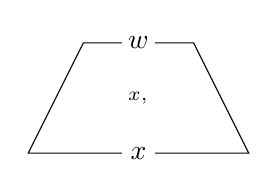
\begin{tikzpicture}[scale=0.7]
\draw (-0.3,-2) -- (-2,-2) -- (-1,0) -- (-0.3,0);
\draw (0.3,-2) -- (2,-2) -- (1,0) -- (0.3,0);
\node (top) at (0,0) {$\un{w}$};
\node (mid) at (0,-1) {$\LL_{\un{x}, \eb}$};
\node (bot) at (0,-2) {$\un{x}$};
\end{tikzpicture}
\end{array}
\]
where the upper expression is always reduced.

Now let $\un{x}$ and $\un{y}$ be fixed expressions. 
Following Libedinsky, we introduce the \emph{double leaves} morphism
\[
\LLL_{w,\eb,\fb} \define 
\begin{array}{c}
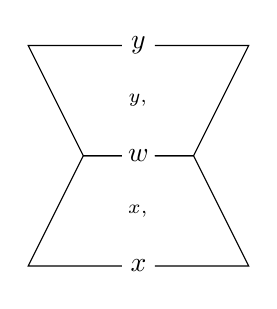
\begin{tikzpicture}[scale=0.7]
\draw (-0.3,-2) -- (-2,-2) -- (-1,0) -- (-0.3,0);
\draw (0.3,-2) -- (2,-2) -- (1,0) -- (0.3,0);
\draw (-0.3,2) -- (-2,2) -- (-1,0) -- (-0.3,0);
\draw (0.3,2) -- (2,2) -- (1,0) -- (0.3,0);
\node (top) at (0,2) {$\un{y}$};
\node (mid) at (0,1) {$\oLL_{\un{y}, \fb}$};
\node (top) at (0,0) {$\un{w}$};
\node (mid) at (0,-1) {$\LL_{\un{x}, \eb}$};
\node (bot) at (0,-2) {$\un{x}$};
\end{tikzpicture}
\end{array}
\]
where $\oLL_{\un{y}, \fb}$ denotes the vertical flip of a light leaf morphism, and $\eb$ (resp. $\fb$) is a subexpression of $\un{x}$ (resp. $\un{y}$) which expresses $w$. Hence $\LLL_{w,\eb,\fb}$ is a morphism $B_{\un{x}} \to B_{\un{y}}$. Consider the set
\[
\LLL_{\un{x}, \un{y}} \define \bigcup_{w \in W} \{ \LLL_{w,\eb,\fb} \; | \; \eb \in M(\un{x}, w), \fb \in M(\un{y}, w)\}
\]
where, $M(\un{x}, w)$ denotes the set of subexpressions of $\un{x}$ expressing $w$. Our main theorem is then the following:

\begin{thm} $\LLL_{\un{x},\un{y}}$ is an $R$-basis for $\Hom_{\DC}(B_{\un{x}}, B_{\un{y}})$. \end{thm}

The proof of this theorem is pure diagrammatic algebra. Unfortunately it is quite convoluted. It has the following consequences:
\begin{enumerate}
\item Under very general assumptions one has a functor $\DC \to \SBim$ (we defined this functor earlier under the assumption that $2$ was invertible).  If the category of Soergel bimodules is well-behaved (i.e. if the Soergel Categorification Theorem holds) then this functor is an equivalence of monoidal categories.
\item Soergel bimodules play an important role in modular representation theory \cite{Soergel, FiebigJAMS}.
Here it is desirable to have versions over fields of positive characteristic and local rings. One can define the diagrammatic category over very general rings. For example, if $W$ is crystallographic then one can define the diagrammatic category over $\ZM$. Over a complete local ring the indecomposable objects in the diagrammatic category are parametrized (up to shift) by $W$, and the split Grothendieck group always categorifies the Hecke algebra. This gives a new proof of Soergel's Categorification Theorem whenever Soergel bimodules are well-behaved, and suggests that the diagrammatic category is the correct replacement when they are not.
\item The category of Bott-Samelson bimodules is a cellular category, with cells parametrized by $w \in W$, and with cellular basis given by a fixed choice of light leaves morphisms. In particular, the endomorphism ring of any Bott-Samelson bimodule is a cellular algebra.
\end{enumerate}


% \subsection{Applications of Soergel calculus in representation theory}

% We believe that the generators and relations established in this paper will find important applications in representation theory. Let us mention briefly two applications which the theory has already found:
% \begin{itemize}
% \item In \cite{EWHodge} the authors propose an algebraic proof of the Kazhdan-Lusztig conjecture, and a proof of the Kazhdan-Lusztig positivity conjecture. Although \cite{EWHodge} does not use the results of this paper, they allowed the authors to perform many calculations which would have been extremely difficult otherwise. The intuition gained from examples was indespensible for \cite{EWHodge}. In a forthcoming paper we hope to explain how to translate the results of \cite{EWHodge} into the language of this paper, and explain the Hodge theory of Bott-Samelson bimodules.
% \item One may use the results of this paper to find examples of torsion in the intersection cohomology of Schubert varieties. The second author has recently used these techniques to give counter-examples to Lusztig's conjecture on the modular characters of reductive algebraic groups. These examples also lead to counter-examples to the James conjecture.
% More generally, it seems likely that one can use this calculus to give character formulas that are valid independtly of Lusztig's conjecture (this idea goes back to Soergel).
% \end{itemize}

\subsection{Organization of the paper}

This paper contains three parts. 

\begin{description}
\item[Part \ref{pt:background}] The first two sections give background on the Hecke algebra and Soergel bimodules.
\begin{description}
  \item[Section \ref{sec-hecke}] We recall the Hecke algebra, Kazhdan-Lusztig basis and Deodhar's defect formula.
  \item[Section \ref{sec-sbim}] We define standard and Soergel bimodules, state Soergel's categorification theorem and discuss realizations and localization.
\end{description}
\item[Part \ref{pt:diagrammatics}] In the next two sections, we define the diagrammatic categories.
 \begin{description}
 \item[Section \ref{sec-diagstd}] We define the diagrammatic presentation of standard modules.
 \item[Section \ref{sec-diagsbim}] We recall results of \cite{EDihedral} and define the diagrammatic category of Soergel bimodules.
  \end{description}
\item[Part \ref{pt:proofs}] In the last two sections we study the diagrammatic categories and prove the equivalence to Soergel bimodules.
\begin{description}
  \item[Section \ref{sec-LLL}] We define Libedinsky's light leaves and double leaves morphisms in the diagrammatic setting. We state the theorem that double leaves span, and deduce the main theorems of the paper.
\item[Section \ref{sec-LLLproof}] We prove that double leaves span.
  \end{description}

\end{description}

\subsection{Acknowledgements} Both authors would like to thank Mikhail Khovanov for encouraging and supporting their collaboration. The second author would like to thank Nicolas Libedinsky and Rapha\"el Rouquier for emphasising the importance of generators and relations, and Jean Michel for help speeding up his programs.